\documentclass{article}
\usepackage[utf8]{inputenc}
\usepackage{lstautogobble}
\usepackage[export]{adjustbox}
\usepackage{graphicx}
\usepackage{changepage}
\usepackage{listings}
\usepackage{amsthm}
\usepackage{subcaption}
\usepackage{amssymb}
\usepackage{titlesec}
\usepackage{hyperref}
\usepackage{lscape}

%Command to change name of table of contents
\renewcommand*\contentsname{Table of Contents}

%Command to start sections on new pages
\newcommand{\sectionbreak}{\clearpage}

%Create a new "Unlabeled section" that will be added to toc but not printed
\newcommand{\unlabeledsection}[1]{%
 \clearpage
  \par\refstepcounter{section}% Increase section counter
  \sectionmark{#1}% Add section mark (header)
  \addcontentsline{toc}{section}{\protect\numberline{\thesection}#1}% Add section to ToC
  }
  
\emergencystretch=1em

\title{OpenUAS:\\Spring 2020 Final Report }
\author{ }
\begin{document}


%%TITLE PAGE%%
\maketitle

\newpage

%%TEAM PAGE%%
\begin{center}
\Large \textbf{The OpenUAS Team}

\vspace{1cm}

\large{
Hazel Ambort\footnote[1]{ISU Department of Materials Science and Engineering}\\ John Botsford\footnote[2]{ISU Department of Aerospace Engineering}\\ William Burken\footnote[3]{ISU Department of Mechanical Engineering}\\ Ellie Diersen\footnotemark[2]\\ John Edgren\footnotemark[2]\\ Abigail Gries\footnotemark[2]\\ Nick Hendrickson\footnotemark[2]\\ Chris Johannsen\footnote[4]{ISU Department of Electrical and Computer Engineering}\\ Stephanie Jou\footnotemark[2]\\ John Levandowski\footnotemark[2]\\ Alex VandeLoo\footnotemark[2] \footnotemark[4]\\
}\par

\end{center}

\newpage

%%TABLE OF CONTENTS%%

\tableofcontents

%%PROJECT OVERVIEW%%
\section{Project Overview}

\subsection{Purpose}
Currently, there are no open-source unmanned aerial systems (UAS) which are fixed-wing and conceptually available to the general public. There are some similar UAS which are available to the public, but they must be purchased and are not open-source. OpenUAS is producing an open-source, commercial off-the-shelf (COTS) UAS that can be used for educational and research purposes, and it will only consist of components available to the general public, including open-source software.\\\\
Dr. Kristin Rozier, assistant professor within Iowa State's Department of Aerospace Engineering, is the PI on the project. One of her main research areas is system health management for autonomous UAS. Therefore, one of the primary goals for this project is to act as a test bed for her research. As the UAS is also intended to be reconfigurable, it is the end goal that the design can be used in additional research areas as well. Finally, the OpenUAS project is intended to be an educational module for advanced high school and college organizations.\\\\

\subsection{Scope}
In order to develop an open-source, COTS UAS for educational and research purposes that is free and available to the general public, a list of objectives, deliverables, and constraints were identified. The following section will provide an overview of these lists.

\subsection{Objectives}
\begin{enumerate}
\item Create an open-source, affordable, COTS UAS for educational and research flights
\item Provide full documentation of the conception, design, and testing of all systems
\item Act as a test bed for Dr. Rozier's system health management experiments
\item Be easily launched and not require a runway for takeoff or landing. 
\item Be piloted by students and hobbyists
\item Be reconfigurable and support additional components
\end{enumerate}

\subsection{Deliverables}
\begin{enumerate}
\item A functioning design and prototype of a UAS
\item Relevant tools for piloting the UAS from the ground
\item Extensive documentation of the design process
\item Extensive documentation of the manufacturing process
\item Extensive documentation on proper use and safety
\end{enumerate}

\subsection{Constraints}
\begin{enumerate}
\item COTS components
\item Affordable components
\item Easily duplicated components (e.g. all 3D printed parts can be reasonably produced by hobbyists)
\item All components should be reasonably safe (e.g. battery)
\end{enumerate}

%%RELATED WORK%%
\section{Related Work}
\noindent Currently, there are very few comparable fixed-wing UAS. The United States uses UAS such as the RQ-14A Dragon Eye and RQ-11B Raven in its military. Although these UAS are similar in size and weight to the OpenUAS team's target design, the technology and capabilities of these systems are much more advanced, and as such, the budget well exceeds the team's overall budget.\\

\noindent The University of Virginia created the Razor, a small fixed-wing UAS for the Department of Defense. This UAS has a flying wing design and utilizes an Android phone as the main processor. The Razor is of similar size, weight, and performance of the team's target design. One main difference in this system is that it is entirely 3D printed. The team plans on utilizing 3D printing, but not to the extent of the Razor design.\\

\noindent The Albatross is a commercial UAV produced by Applied Aeronautics. Although this aircraft is larger than the team's target design, its performance and low-cost are comparable to the team's goals. This UAV is described in more detail later in the paper, as the team purchased and is beginning to study this design. \\


%%STATUS%%
\section{General Information}

\subsection{Status}
During the Fall 2019 semester, the OpenUAS team built a complete UAS prototype as shown in Figure \ref{2019_model} below. Flight testing for this model occurred during the end of the fall semester and carried over to the beginning of the Spring 2020 semester. Unfornuately, these flight tests were unsuccesssful as the UAS was unable to take-off. Multiple factors were suspected to contribute to the unsuccessful flight tests. The W/S ratio for the wing was likely too large causing the stall speed to be too high; therefore, the aircraft could not get past this stall speed to achieve flight. Additionally, the motor was likely undersized and could not provide sufficient thrust at take-off. Although this model never flew, it served as example of what worked and what could be improved upon for this semester's design.

\begin{figure}[hbt!]
\centering
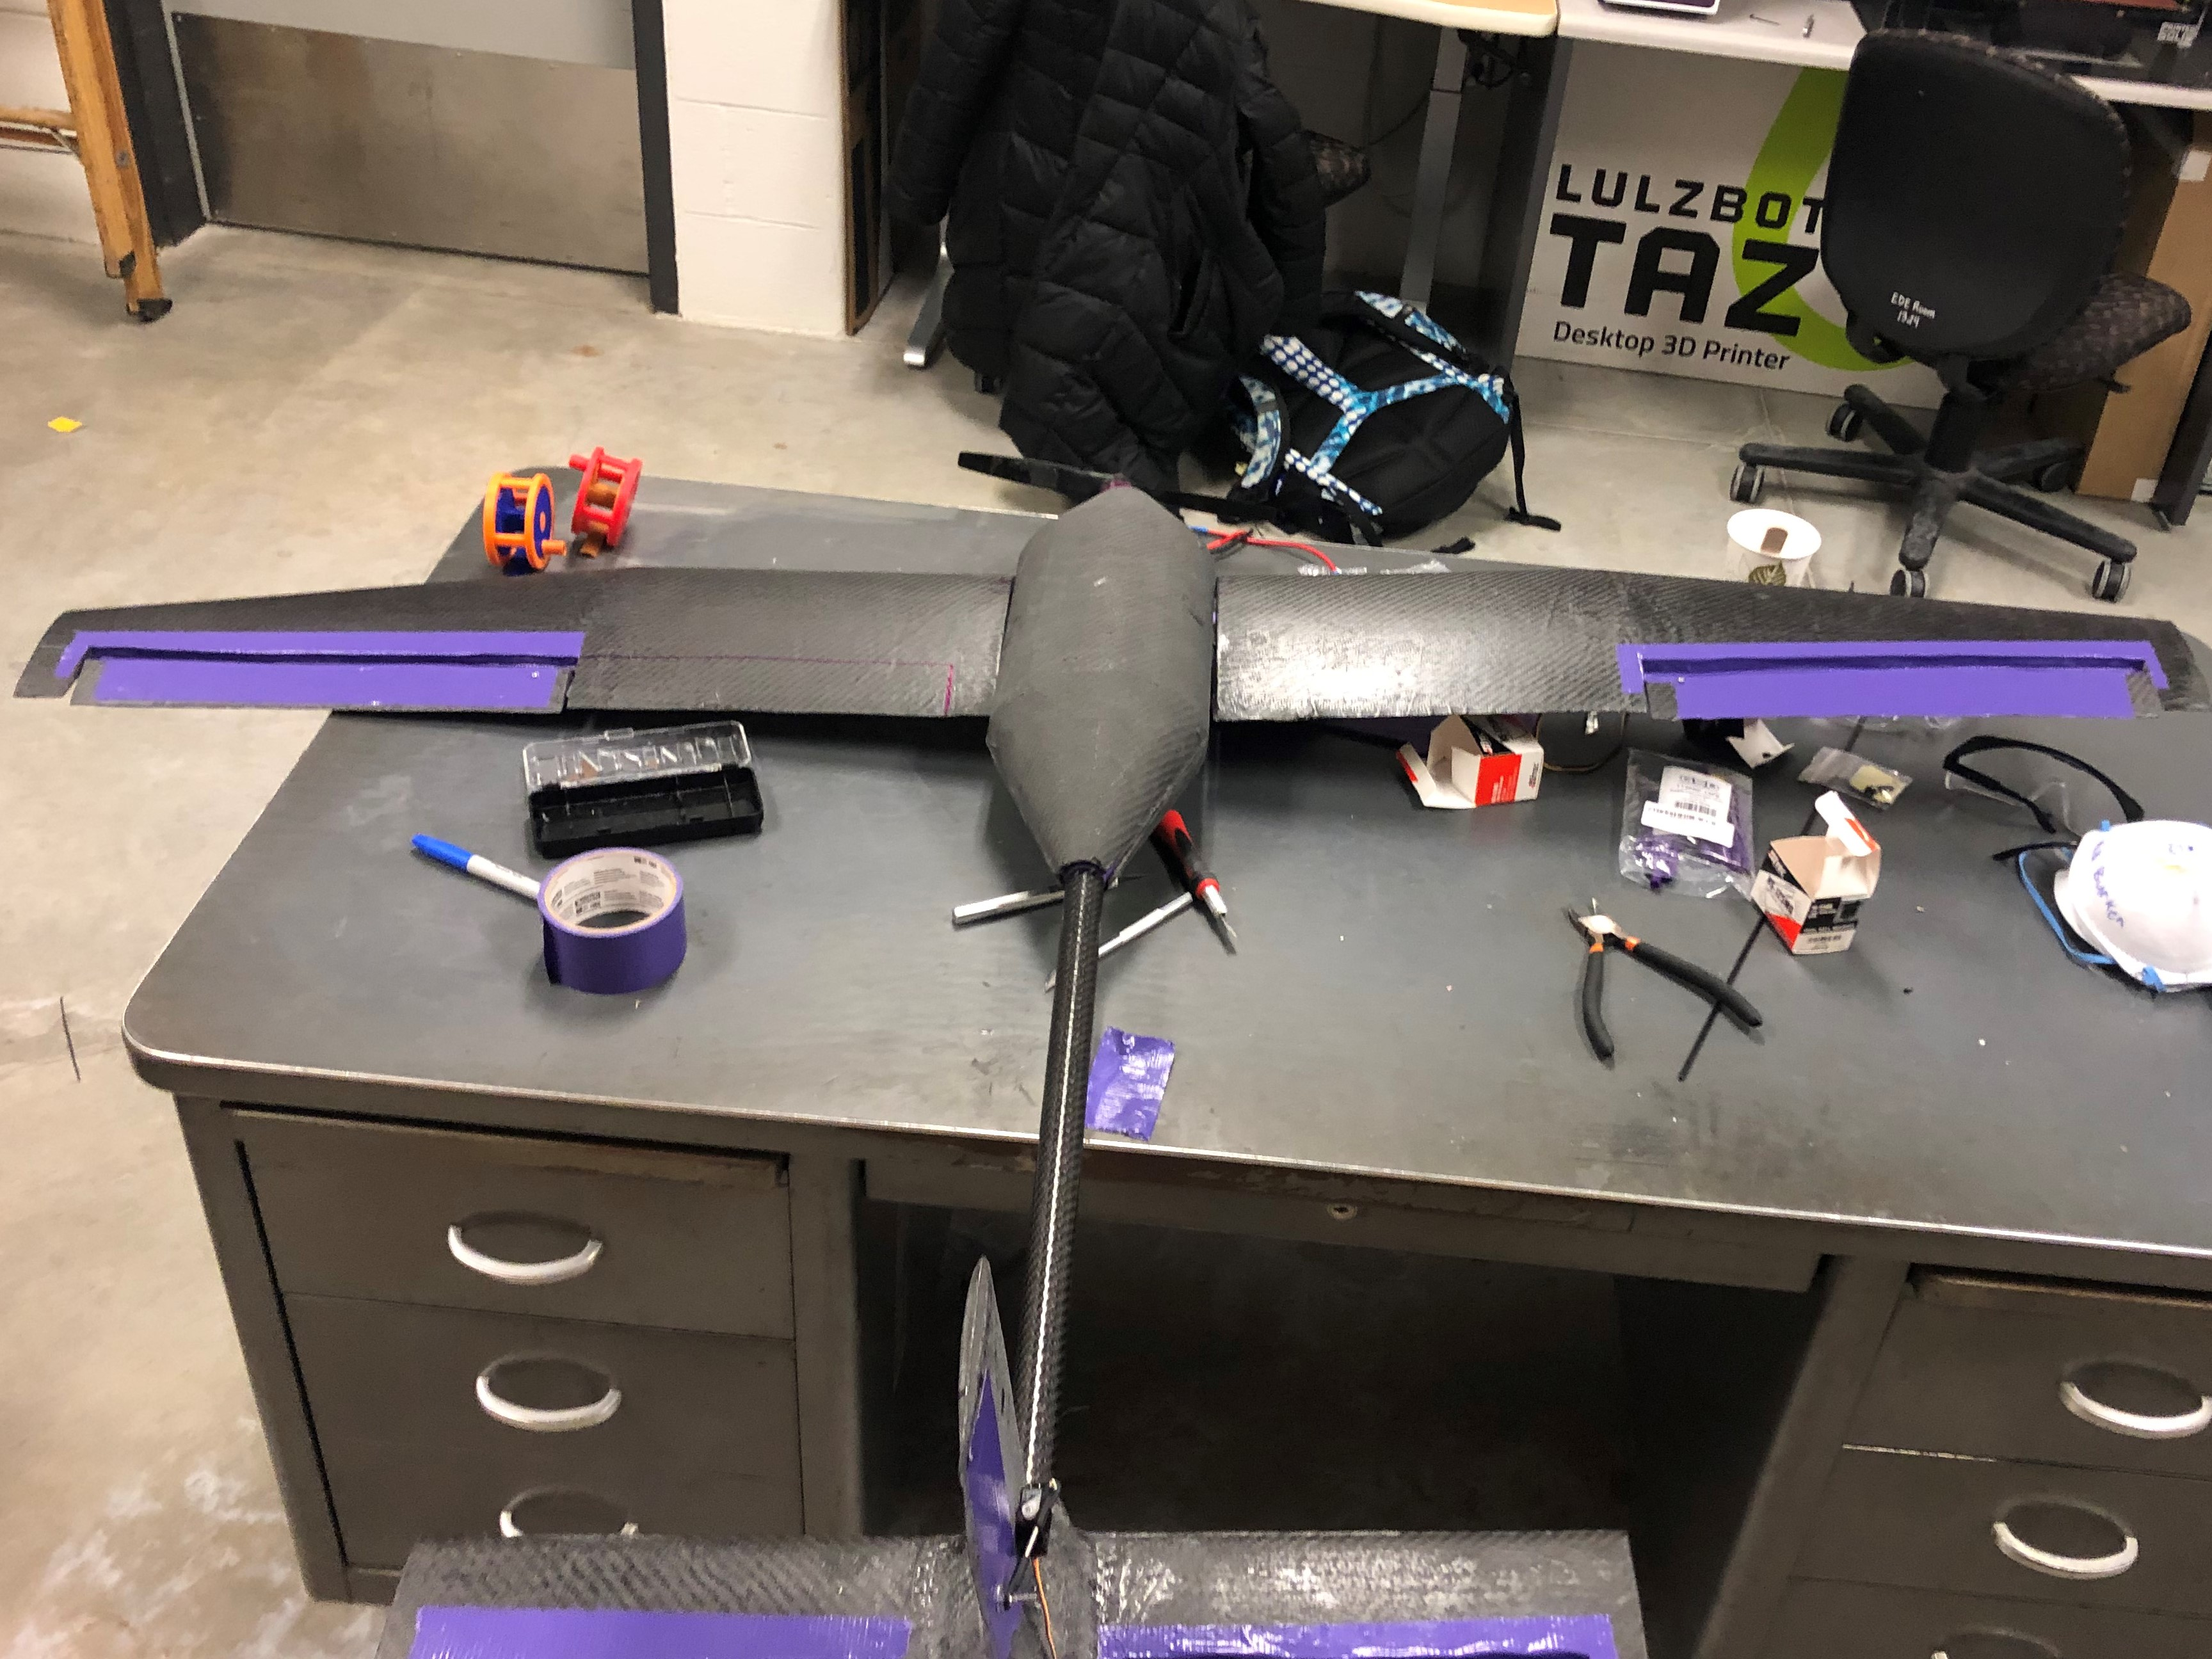
\includegraphics[width=0.5\textwidth]{OpenUAS_Fall2019_Model.jpg}
\caption{Fall 2019 OpenUAS Prototype}
\label{fig:2019_model}
\end{figure}

The first couple weeks of the Spring 2020 semester were spent getting the new team members up to speed on the project and flight testing the previous model. After it was determined that the previous model would no longer fly, design changes based on the flight test failures were incorporated into this semester's design. Specifically, the wing size was increased (both chord and span), the target weight was decreased by redesigning the fuselage, and new electronics were chosen (including a more powerful motor to increase thrust). The team intended to begin the manufacturing of this Spring 2020 model after Spring Break, but the COVID-19 pandemic caused delays in this progress. Some foam parts were CNC'd, but the composite work and assembly was not able to take place this semester. 

The team intends to continue the manufacturing process into the Fall 2020 semester. Composite work, part assembly, and integration with electronics will ideally take place within the first several weeks of the semester. After manufacturing and intergration is completed, the team will flight test this new model.  This work will be aided by new team members joining in the fall.

\subsection{Team Organization}
The flowchart (Figure ) on the next page shows the organizational structure of the OpenUAS team. The membership of the team is changing every semester as new students join the team and previous members graduate or take a leave of absence. Many team members are graduating this school year, so it was necessary to fill these positions on the team. Interviews are still on-going for the Structures and Electrical/Software teams, so it is likely that new members will be added to the team before next semester.\\\\

\newpage

\begin{landscape}
\begin{figure}[hbt!]
\centering
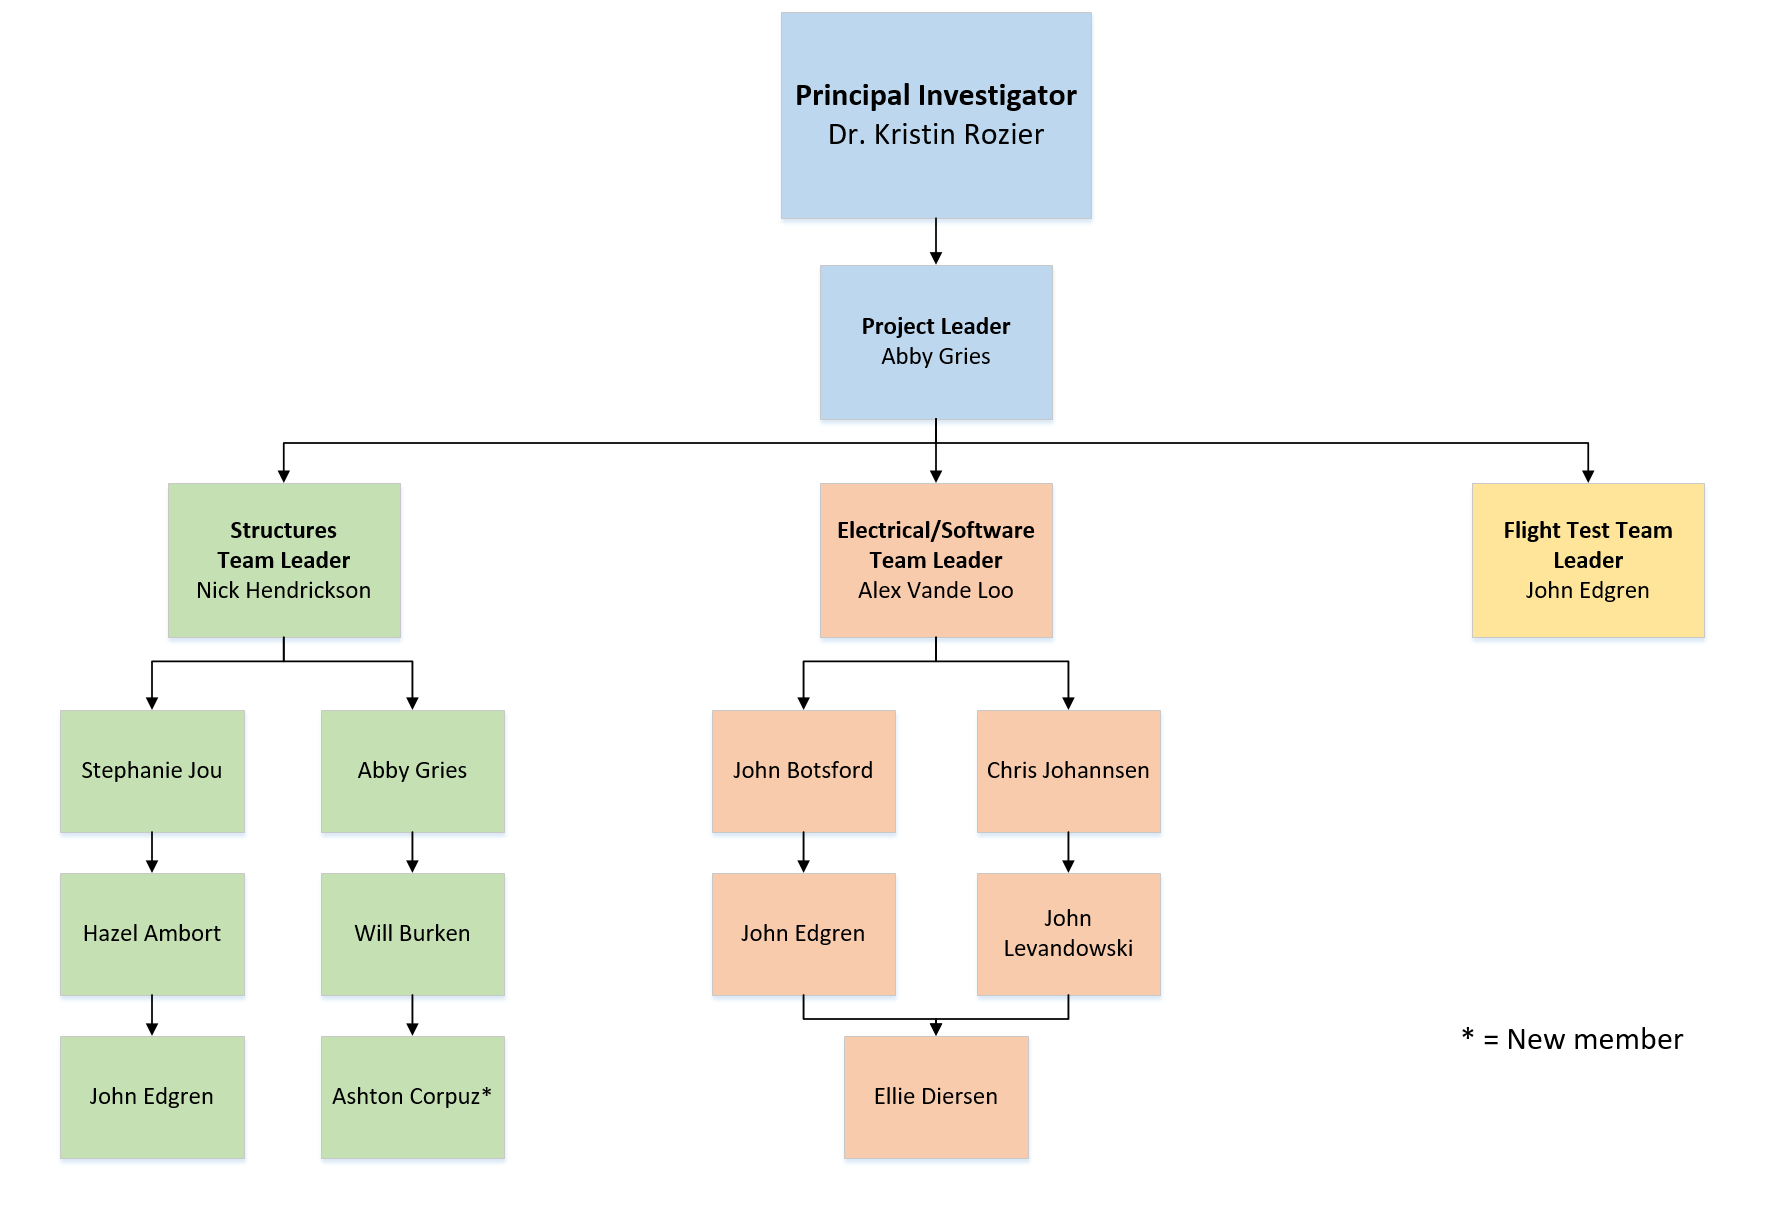
\includegraphics[scale=0.75]{TeamOrganization_Spring2020.png}
\caption{Fall 2019 OpenUAS Prototype}
\label{fig:2019_model}
\end{figure}
\end{landscape}

\newpage

\subsection{Documentation}

Varying forms of documentation were developed to assist with tracking the vision, objectives, high-level project plan, and weekly progress and goals. The documentation is intended to not only support the systems engineering aspect of the project, but also serve an educational purpose by assisting future users who would like insight into what efforts and decisions were made to bring OpenUAS from a concept to a reality. Additionally, everyone on the team keeps their own weekly and semester progress documentation to maintain goals and the vision for every subgroup within the OpenUAS team. 

\begin{enumerate}
\item \textbf{Project Charter}\\ This one-page document was created at the conception of the project and is intended to help provide a broad overview of the project. The Project Charter lays out the scope and purpose of the project. Additionally, the project objectives, deliverables, and constraints that were mentioned earlier in this paper come from the Project Charter. 
\item \textbf{Team Organization}\\ This flowchart shows the organizational structure of the OpenUAS team. The overall team is broken down into three sub-teams: electrical, structures, and flight test. These sub-teams have team leaders and members. The overall project has a project leader. This will change each semester as students join or leave the team. 
\item \textbf{Weekly Meeting Agenda}\\Each week before the team meeting, team leaders update the Weekly Meeting Agenda. This document details the progress made for the week and the goals for the next week. Additionally, team leaders can request assistance through this document and the agenda for the meeting is set by the project leader. Attendance for each meeting is also taken in this document. 
\item \textbf{Requirements}\\ The requirements document is an extensive, volatile artifact that has been developed since the beginning of the project. Originally, our primary requirements were high-level and directly traceable to the overall project goals. Now, as we begin to make decisions about what our design will look like, the requirements have evolved to become more detailed. For the sake of making requirements easier to read and understand, we chose to use the EARS \cite{Terzakis2013} requirements syntax. These requirements will be updated again in the Spring 2020 semester as the next design iteration begins. 
\end{enumerate}

\subsection{Lab Set-Up \& Organization}
\noindent The lab originally started out with no equipment or tools available for our project. Throughout the last school year, orders had been placed for tools and other items needed in order to ensure a work space that has all tools needed for successful progression of this project. This last semester has built off what was completed before, adding new equipment, rearranging tables and desks to provide more surface area in the lab for various projects, and adding more tool locations for easier access to common tools.  Because we are working within a large organization, special documentation and communication must be done in order to acquire the parts needed for the lab. This includes confirmation of successful retrieval of parts and checking if damage was done to them. If damage is found, proceeding with the proper return process and notifications so everyone knows how parts are moving about. If an item is not the item we purchased (e.g. a different sized cartridge for a label printer) we send it back to the individual keeping track of our orders and have them re-order the right equipment. The final goal is to have a lab outfitted in such a way that it can complete any of the tasks designed for the project with exceptions to precision machining and other similar processes.\\


\subsubsection{3D Printer - LulzBot Taz 6}
The LulzBot Taz 6 3D printer was not used this semester as no manufacturing work took place. Additionally, one of the flaws of the Fall 2019 model was that it was too heavy because of the amount of 3D printed components used on it. In the future, it is likely that the 3D printer will only be used for small and/or limited components aboard the UAS. If the printer is utilitized in the future, it's firmware and the CURA Lulzbot software should still be updated regularly as there are some software/firmware issues with the LulzBot Taz 6. It will also be essential to continue to take care of the printer through updates, bed maintenance, and part replacement to keep the printer in the best shape possible. 

%%INSPIRATION: THE ALBATROSS%%
\section{Primary Inspiration: The Albatross UAV}
\noindent The Albatross UAV is a commercial product of Applied Aeronautics. The team purchased this model in the fall of 2017 to study the documentation, the ease of construction, and the flight characteristics of this model. The Albatross UAV has a wingspan of approximately 9.8 feet and is advertised to carry over 4.4 kg of payload over 4 hours. The Albatross is capable of a maximum 90 MPH speed and a cruise of 40 MPH. This UAV has so far been extremely beneficial in the lessons learned from purchasing, documentation, and the construction of UAS in general. 

\subsection{Construction and Progress}
The Albatross was constructed by the end of December in 2018 but has not been flown. The Albatross construction was conducted over two semesters for the OpenUAS team due to severe lack of documentation from the supplier, Applied Aeronautics. From the construction process, the OpenUAS team learned quite a lot from setting up servo connections, the internal organization, drilling into certain components, and in how to better document build processes for future designs. 

\subsection{Looking forward}

While no progress has been made this semester on the Albatross, the team does plan to fly it in the future. This will be useful in testing things like flight modes, gathering flight data, and providing insight into further advancements that can be made for the OpenUAS design. This next semester, in coordination with continuing to fly the OpenUAS models, the OpenUAS team hopes to maintain the Albatross as a flight ready vehicle for any flight-testing needs. 

%%SYSTEM ARCHITECTURE AND PROGRESS%%
\section{OpenUAS System Architecture \& Progress}
This semester the OpenUAS team split into three sub-teams: electrical/software, structures, and flight test. The structures team was primarily responsible for the airframe design, simulations and calculations (including CFD, center of gravity, stability, etc.), and manufacturing process. The electrical team worked on the hardware, wiring, and software. The flight test team created preflight procedures, ground tests, and the flight tests for the UAS. The following sections describe in detail the work performed by each sub-team this semester. UAS1 refers to the UAS built this semester.  

\subsection{Structures Team}
This section will discuss the design process and decisions made with respect to the OpenUAS prototype that was built this semester.

\subsubsection{Design}

\textbf{Things to include here: design changes from previous work, solidworks models, airfoil analysis, stability analysis, center of gravity work, etc. Can make more subsections or subsubsections as you see fit.}

\paragraph{Design Changes from Previous Work}
Comparing both the Spring 2020 and Fall 2019 designs, a number of changes were made to address some of the problems encountered during the fall. The main concerns and decisions made are listed below.\\

\begin{enumerate}
  \item{Center of Gravity Location}\\
  During the Fall 2019, there were problems with the location of the center of gravity that was not close to the wing's quarter chord. This caused problems during the test flights since it was too much towards the front. To address this issue and prevent it from happening this semester, the wings were placed at the back of the fuselage instead of the middle.\\
  
  \item{Mounting of the Wings}\\
  During several test flights last semester, the UAS crashed. Because of this, the wings came apart on many ocassions. These resulted in team members making repairs and looking for ways to patch up the wings back to the fuselage. These fixes were done with duct tape, epoxy, and carbon fiber composite sheets. These elements added weight, making the UAS heavier and therefore, changing the properties of the UAS.\\
  To solve this issue, the wings were set farther to the back of the fuselage and high mounted. High mounted wings enable easier handling of the wings by eliminating the connection points that were dealt with before. This also eliminates the need of the 3D printed parts used in the previous iteration which added up quite some weight to the UAS. With high mounted wings, it is easier to remove them and if they break, it is easier to replace them. This also creates another access point to the fuselage for hadling the electronics.\\
  
  \item{Performance Increases}\\
  The overarching flaw of the Fall 2019 design was a lack of performance; the UAS was overweight for the amount of lift and thrust it could produce, and as a result it could not gain flying speed from a hand-launch. To mitigate these issues in the Spring 2020 UAS design we chose to focus on weight reduction and lift and thrust increases. To reduce weight we will use fewer or no 3D-printed parts and utilize foam wings and tail surfaces with at most a single layer of carbon fiber of fiberglass for strengthening. Additionally, the size of the fuselage has been decreased, and we will utilize a smaller, lighter, battery. To increase lift, the wing was redesigned longer in span and chord length, and with no taper. Finally, a larger motor was purchased to increase the thrust produced and bring the thrust-to-weight ratio closer to 1:1. \\

\end{enumerate}

\paragraph{Solidworks Models}
This semester Solidworks was again used to design the entire UAS before it was built and for the purpose of running Computer Analysis Simulations. All members of the Structures Team contributed to the Solidworks design. As the design went through many iterations, the structures team endeavored to build every part in a way that could be easily changed. The greatest challenges with the Solidworks design were creating a fuselage shape that would meet all of our requirements and determining how to secure various components to the airframe. Initial iterations utilized an oval-shaped curved fuselage, however, the requirement for ease of access to the electronics located in the fuselage led us to make a roughly rectangular fuselage shape. The rectangular fuselage will be able to more easily accept an ''Electronics Sled'' with all electronics components on it as well as the Nose Cone and electric motor attached to the front.\\

Securing components to the airframe was another challenge that we handled in multiple ways. The tail surfaces will utilize thin rods that add support to the foam surfaces and extend through the tail-rod for attachment. The wing will be secured with 4 nylon bolts into the fuselage which will allow it to be easily removed for transport. Attaching the electronics sled may be accomplished with an additional 4 nylon bolts, however, this design is yet to be solidified. The tail-rod may be fixed into the rear of the fuselage or attached in such a way that it can be removed for transport.\\

Compared to the previous design, the Solidworks model this semester included a higher-mounted wing that incorporated two degrees of dihedral for increased stability. The tail-rod was also located at the top of the fuselage to allow extra clearance for hand-launching or a ground-launching mechanism. Finally, larger control surfaces were incorporated for increased controllability and responsiveness.\\


\paragraph{Airfoil Analysis}
For this semester, the airfoil used was not changed from the previous semester. The reason being that since there was no data that suggested any problems with the airfoil chosen. Recalling that the problem on the UAS last semester was the center of gravity, the ClarkY airfoil was still used. The plan is to keep using this airfoil unless data or calculations suggest that not enough lift is generated when using this airfoil.\\
However, there was some analysis done with this airfoil and quite some information used from previous semesters for this. XFLR5 was used to obtain some lift coefficient curves and predict the aerodynamic variables. There was some sizing done depending on the values obtained from XFLR5. This would also affect the distance between the tailboom and the fuselage.\\

\paragraph{Stability Analysis}
The open-source computer program, AVL, was used to analyze the stability of the UAS. After an initial model was created in Solidworks, AVL was used iteratively to size the tail appropriately. The distance between the center of gravity of the entire UAS and the stabilizers as well as the stabilizers' chord and span were changed during this process. In the end, a static margin of approximately 11\% was achieved with the final tail configuration, which was in the recommended range for comparable UAS designs. AVL was also used to size the elevator and rudder to ensure proper pitch and yaw control during flight. The maximum elevator deflection for the design was determined to be -12.5 degrees. This is within the obtainable range for the servos. 

\paragraph{Center of Gravity}
Because of the issues that we had last semester with the center of gravity, we completed a center of gravity simulation on our new design this semester. SolidWorks was used for calculating and identifying the center of gravity for the new design. This process took several weeks so that we could ensure that the simulation was completed correctly. The materials for each component of the new design were added to each piece. We tried to obtain and use materials as close to the materials that we decided to use for the real model. The masses for the electronic components were also obtained to add point masses into the simulation for accuracy.\\

Once the materials and masses were added into the simulation, the analysis was ran to determine where the center of gravity would be. The model included the wings, tails, fuselage, and most of the electronics. The model did omit wiring and some smaller masses. These smaller masses were omitted because they would not have significantly contributed to the location of the center of mass.\\

The simulation was ran, and the center of gravity looked to be approximately a quarter of the chord length. This was thought to be about the right position and what was necessary for our design. Several members continued to check and correct the weights in the simulation, and the center of gravity remained in the same position. The team generally agrees that the current position of the center of mass is sufficient for success of our new iteration.\\

\subsubsection{Computer Simulations}


\subsubsection{Manufacturing}
This semester, the manufacturing process was not done properly due to the transition to remote work. Before Spring Break, some parts such as the fuselage and the tail cone were manufactured with the CNC machine by the structures team lead using Mastercam. This was tried since Andrew Jordan from the Aerospace Department did not give a specific timeline as to when the pieces could be ready for and he had a backlog with Senior Design parts to prepare. To reference, Andrew Jordan has been the person to go to for the printing and manufacturing of the different pieces for the UAS. \\
After the pieces were print by the team lead, several team members proceeded to sand the pieces preparing them for lay-ups with carbon fiber. Some other pieces such as the wings were not manufactured since they were going to require more than one piece of foam. For cleaner pieces to be print out, the structures team was able to reach out to Andrew Jordan once again this semester. Given the current circumstances (remote work transition), he was able to print out all the pieces for the UAS. \\
Moving forward, the team will proceed to complete the lay-ups for this iteration and assembly of the UAS during the start of the fall semester later this year. The objective is to completely finish the iteration by assembling the craft, performing test flights, and analyzing the data.\\

\subsubsection{Launch System}
Will


\subsection{Electrical/Software Team}
This section will discuss the internal components and software that have been used for the OpenUAS prototype that was worked on this semester.

\subsubsection{Software}
This semester we looked into setting up a custom airframe setup for our UAS, which will allow us to streamline the setup for new Pixhawks. This means that setting up things such as ailerons on two channels, control surface trims and directions, and any other parameter that has to be set in QGroundControl can be preset on the initial boot of the system. Due to Covid-19, only one attempt was made at loading a custom airframe to the Cub, which was unsuccessful. However, much was learned about how the pixhawk firmware works, such as how to modify the boot script on the pixhawk, how to change system parameters, and how to write the .MIX files the Pixhawk uses for controlling servos and motors. It was also discovered how to interact with the Pixhawk through it's comamnd line terminal, which will be very useful in trouble shooting future attempts at implementing an airframe.\\ \\

With the virtual work option this semester, documentation was completed in regards to a few different softwares. The first being QGroundControl; a document detailing how a new Pixhawk4.0 can be fully set up through QGC. This is a detailed process that connects to two documents that were created in setting up the Taranis controllers. The first of these is a Taranis Model Set Up document that walks a new user through setting up a proper model on the controller and assigning the correct channels based on the specific airframe that they want to fly. Additionally, a flight mode set up document for the Taranis controller was also completed that helps a user create either 3 or 6 flight modes for their model. This uses logical switches on the controller and allows for quick transition between the different flight modes. Finally, an OpenTX companion document was produced that allows the user to create their models and set up their flight modes on this computer software then upload them to the controller so that the manual process of inputing the models can be skipped. Other software documentation completed was in regards to the battery charger. This document sets up basic balance charges and cyclic charging and discharging of LiPo batterries in the lab. In addition to this document, a LiPo battery safety and use document allows an unfamiliar user to understand the basics of LiPo batteries and how they should be handled safely. \\ \\

There was also work put towards the goal of integrating R2U2 with the craft. The C version of R2U2 currently functions statically on the lab Raspberry Pi B+. This means that R2U2 can analyze a set of log data after said data has been collected. In the future, once R2U2 has been developed more, the live version can be worked with. There was also some preliminary work put into finding a way to interace the Raspberry Pi with the Pixhawk as a companion computer so that R2U2 can analyze live data fed from the flight computer. This will be the end goal, and more work needs to be done to get the Pi to communicate with the Pixhawk, specifically with regards to the physical connection. There are many protocols that can be used, however the MAVLink protocol looks the most promising using the serial port on the Pi. \\ \\

The research of different autonomy options began during this semester because the research had progressed far enough in the pixhawk setup of the aircraft, which allowed for the focus on more advanced options. Achieving autonomous flight is done through the Mission Planner setting within QGroundControl. This allows for the design of different missions that will track the vehicle position, its waypoints, and whichever instruments attached to it. There are required parameters for the mission and the UAV that need to be set up including name of mission, bounds, name and type of UAV, initial position, configuration of the UAV, flight profiles, etc. After these are set up, an objective for the UAV to accomplish during the mission can be added. The objective also has required parameters like its name, where the task will take place, what kind of task it is, etc. Within the limits of QGroundControl the options for autonomy are running missions with waypoints, taking a photo or video, taking off or landing, surveying, or controlling altitude. All of this research is described further in depth in the Autonomy Research Document. \\ \\

\subsubsection{Electronics}
This semester the electrical system was able to be revamped in a number of ways. In order to fit in with the new pixhawk 4 that was being used for this iteration of the Iron Bird, the whole system was looked at and assesed to see which parts were necessary and what could be streamlined or removed altogether. One large change that was able to be made was streamlining the servo rail. Here it was found that the BEC contained in the ESC could be used to plug directly in line with the servos to power them. This cleaned up the wiring for the servos and entirely removed one of the BECs. The second redundant BEC was also able to be removed due to an updated PDB for the Pixhawk 4. \\\\
The components used were also able to be updated. After the flight tests last semester and the beginning of this semester, it seemed that one of the problems was the weight being too high coupled with the thrust being too low. This lead the team into thinking about how many of the components might be able to be modified to better suit the project. As it would be difficult to plan for future iterations and adjustments, a range of ESCs, batteries, and motors were ordered. Having these, the team would be able to switch out the components in order to test more designs without needing to just predict or order new parts. \\

Many new components were ordered for the electronics team this semester. The reason for this is to allow the project to continue on with the appropriate materials to create a flying UAS. With the closure of campus, this was an opportunity to sit down and figure out all the compents required for future iterations. Finally, becuase funding will be freezed at the end of this semester it is important to get the materials now. In table \ref{table:order list}, the new components that have been ordered for the electrical team are listed. With these components future iterations of the UAS will be successful and the team will have a some options in choosing various propulsion systems that fit the needs of that specific iteration. Specifically, multiple batteries, ESCs, motors, and propellers were ordered. These propulsion components will not be put together without reason however. Through the use of MotoCalc, a propulsion system performance calculator, the components can be smartly chosen and confidence can be ensured that the chosen propulsion system will provide appropriate thrust for the UAS model, more can be found on this in the propulsion section. Additionally, optimizations can be performed based on the given structure to provide better flight times and ranges. The procurment of these components will drastically enhance the electronics teams' capabilities to provide a working electrical system for the UAS. \\ \\

\begin{table}[h!]
\centering
\begin{tabular}{|c|c|} 
 \hline
 \textbf{Item} & \textbf{Quantity} \\
 \hline
 Pheonix Edge ESC 100A & 1 \\
 \hline
 Hacker A-30-10XL, 900kv & 1 \\
 \hline
 FrSky Neuron ESC 80A & 1 \\
 \hline
Badass 2826-690kv & 1 \\
 \hline
 Badass 3520-560kv & 1 \\ 
 \hline
 Badass 3520-790kv & 1 \\
 \hline
 Badass 3520-970kv & 1 \\
 \hline
 Badass Renegade Seies ESC/BEC Combo, 85A & 1 \\
 \hline
Badass Renegade ESC Programmer LCD & 1 \\
 \hline
Pixhawk 4.0 with wiring package & 3 \\
 \hline
Pixhawk 4.0 Cable Set & 1 \\
 \hline
 Ovonic 4000mah, 50C, 3S Lipo, 280g & 1 \\
 \hline
Ovonic 5000mah, 50C, 3S LiPo, 381g & 1 \\
 \hline
Ovonic 6400mah, 50C, 3S LiPo, 422g & 1 \\
 \hline
Control Horn to Servo Push Rods (2-56 size) & 2 \\
 \hline 
 LiPo Battery Checker/Buzzer & 1 \\
 \hline 
HRB 3000mah, 60C, 4S LiPo, 297g & 1 \\
 \hline
Ovonic 7600mah, 50C, 3S LiPo, 456g & 1 \\
 \hline
Ovonic 3000mah, 50C, 3S LiPo, 193g & 1 \\
 \hline
Control Horns & 2 \\
 \hline
xt60 Connectors & 1 \\
 \hline
12x10-E APC Propeller & 3 \\
 \hline
13x10-E APC Propeller & 6 \\
 \hline
14x10-E APC Propeller & 3 \\
 \hline
14x12-E APC Propeller & 3 \\
 \hline
2-56 Threaded push rod 48 inch & 4 \\
 \hline
Lumenier 35C 2250mah 170g 3S & 1 \\
 \hline
E-Flite Apprentice STS Smart Trainer  & 1 \\
 \hline
Thin Wing HS-125MG Servo & 2 \\
 \hline
\end{tabular}
\caption{New Electronics Components Ordered}
\label{table:order list}
\end{table}

\subsubsection{Propulsion}
After the first couple flight tests, it seemed that the current motor and propellor were not the best choice for the UAS. By using MotoCalc, a new motor and propellor combination was selected to provide more thrust for the craft. Following this line of thinking and looking forward to furute iterations of the UAS, a number of new propellors and motors were ordered using the same software to help the selection process. This was done so that if a similar problem is found in the future, new motors and props can be quickly and easily tested to find the best combination for that version of the UAS. \\ \\

\subsection{Flight Test Team}
This semester the Flight Test team produced several documents, performed two unsuccessful test flights, and one successful test flight. Documents produced include a document outlining appropriate weather requirements and minimums for all UAS flights, a “New Pilot Training Manual” for the purpose of outlining specific steps and methods of learning how to fly a UAS, and a document outlining the steps to link two Taranis controllers in a “Trainer mode” for the purpose of training a new UAS pilot. Additionally, a UAS flight log was created as a spreadsheet for the use of documenting all individual UAS flights in one place, along with links to applicable pre- and post-flight procedures.\\

The first test flight attempt of the semester and fourth flight attempt overall for the first UAS occurred on 2 February 2020. This attempt was unsuccessful due to unexpected electronics malfunctions that had not previously occurred during ground testing. A faulty electronic speed control, or ESC, was determined as the most likely culprit and was replaced before the next flight attempt. The second and final flight attempt of the semester for the first UAS design occurred on 16 February 2020. Using a hand launch technique, the UAS managed to become airborne for only a few seconds before crashing into the ground, impacting with the left wing first, but at a relatively flat pitch attitude. The crash snapped off the left wing and fractured the 3D-printed motor and tail-rod mounts. A lack of sufficient airspeed to fly, resulting in a stall, is believed to be the cause of this crash, which stems from the UAS having a higher-than-optimal weight and not a large enough wing. Between the damage from the last flight attempt and the 2 previous crashes, the team decided not to rebuild the first UAS and instead focus on designing a new UAS taking into account the lessons learned from the first UAS. Both flight attempts of the first UAS this semester were located at a farm field southeast of Nevada, Iowa.\\

A successful test flight of the semester occurred on 10 March 2020 with the Flitetest Cub outfitted with OpenUAS electronics. The Cub was able to become airborne from a ground-takeoff and performed well despite some control trim issues. A low battery forced the Cub to land sooner than planned, however, this flight confirmed the possibility of using the Cub airframe to perform electronics systems tests and checks.\\

Looking forward, the Flight Test team will continue to update flight test procedures and related documents to align with the new UAS and provide clear objectives for future flights. In the next semester, the Flight Test team plans to complete successful flights of the new UAS which will start to include autonomous integration, testing onboard electronics and testing potential structural modifications. Documentation of each flight will provide valuable data for the UAS design to assist the team in our work, and may also give insight to other groups building and flying OpenUAS designs in the future.\\



%%LESSONS LEARNED%%
\section{Lessons Learned}

\textbf{Add lessons learned that you may have}

\begin{enumerate}
\item Start the semester with clear objectives, a practical timeline, and organized deliverables
\item If you're having a problem in setting up controls and telemetry, there is probably a solution through adjusting parameters in QGroundControl
\item Things will very often not work the way you think they will
\item Don't rush a project to the point that the results are sloppy, because it will be time consuming to have to correct later
\item Staying organized, especially with wiring/internal components, is incredibly important
\item It is beneficial to have an understanding of the inventory in the lab; spare components that may be useful could be hidden away somewhere
\item When soldering items, make sure they are soldered to the correct spots
\item Try to complete work early - if you leave it until later in the week or day it can get forgotten
\item While in the design process, constantly verify ease of manufacturing
\item Detail progress, especially in construction and instances of problem solving; it's easy to forget what exactly happened and helps all the team members
\item Servo connections can be simplified; for the OpenUAS, the team should have more organized pathways for wiring or just keep all wiring in the fuselage and have extended servo connections with long rods
\item Update the Cura LulzBot software continuously
\item Splicing can save time on some parts and take more time on others
\item A copy of a tool we already have is never a bad thing when two people need to work on the same project
\item Wear safety equipment 
\item Double check your work
\item Not everything works a second time
\item A clean lab is easier to work in than a messy one
\item Debugging takes time, and even more patience 
\item Never plug things into a system when it is powered on
\item Be careful when powering things up using an external power supply
\item Question why everything is set up the way it is. There may be better ways to do things
\item If you don't know what you're doing, ask someone
\item The internet is your friend
\end{enumerate}

%%LIST OF FUTURE TASKS%%
\section{Future Tasks \& Deliverables}

\textbf{Add future tasks}

\begin{itemize}
\item Continue to test fly UAS number one
\item Complete OpenUAS design number two
\item Test fly the Albatross UAV
\item Add onboard components to test: LIDAR, lights, cameras
\item Create and test a new launch system
\item Conduct a fully autonomous flight
\item Implement the Pixhawk4 and its peripherals into UAS number two
\item Set telemetry callouts from the Taranis automatically
\item Develop smoother assisted flight modes so there is less work required by the pilot
\item Break in all the new batteries by doing 5-7 cycles for each battery
\item Make sure everyone is comfortable charging and storing the batteries
\item Make friends with someone on the Cardinal Flight team in M2i so, if needed, the static thrust stand can be used
\item Run MotoCalc simulations to properly match the batteries with the ESCs, motors, and propellors
\item Store and organize all of the new items arriving at the lab, utilize the order list to make sure everything is still in the lab after the summer
\item \textbf{Actually look at this list at the beginning of next semester to get an idea of things to do in the beginning weeks when everyone has more time}
\end{itemize}


%%REFERENCES%%
\unlabeledsection{References}
\begin{thebibliography}{100}
\bibitem{Terzakis2013} Terzakis, J. (2013). EARS: The Easy Approach to Requirements Syntax. In International Academy, Research, and Industry Association: The Eighth International Multi-Conference on Computing in the Global Information Technology. Retrieved October 11, 2017, from \\\url{https://www.iaria.org/conferences2013/filesICCGI13/ICCGI_2013_Tutorial_Terzakis.pdf}
\end{thebibliography}


\end{document}
